\section{Related Works}

\begin{figure*}[t]
\centering
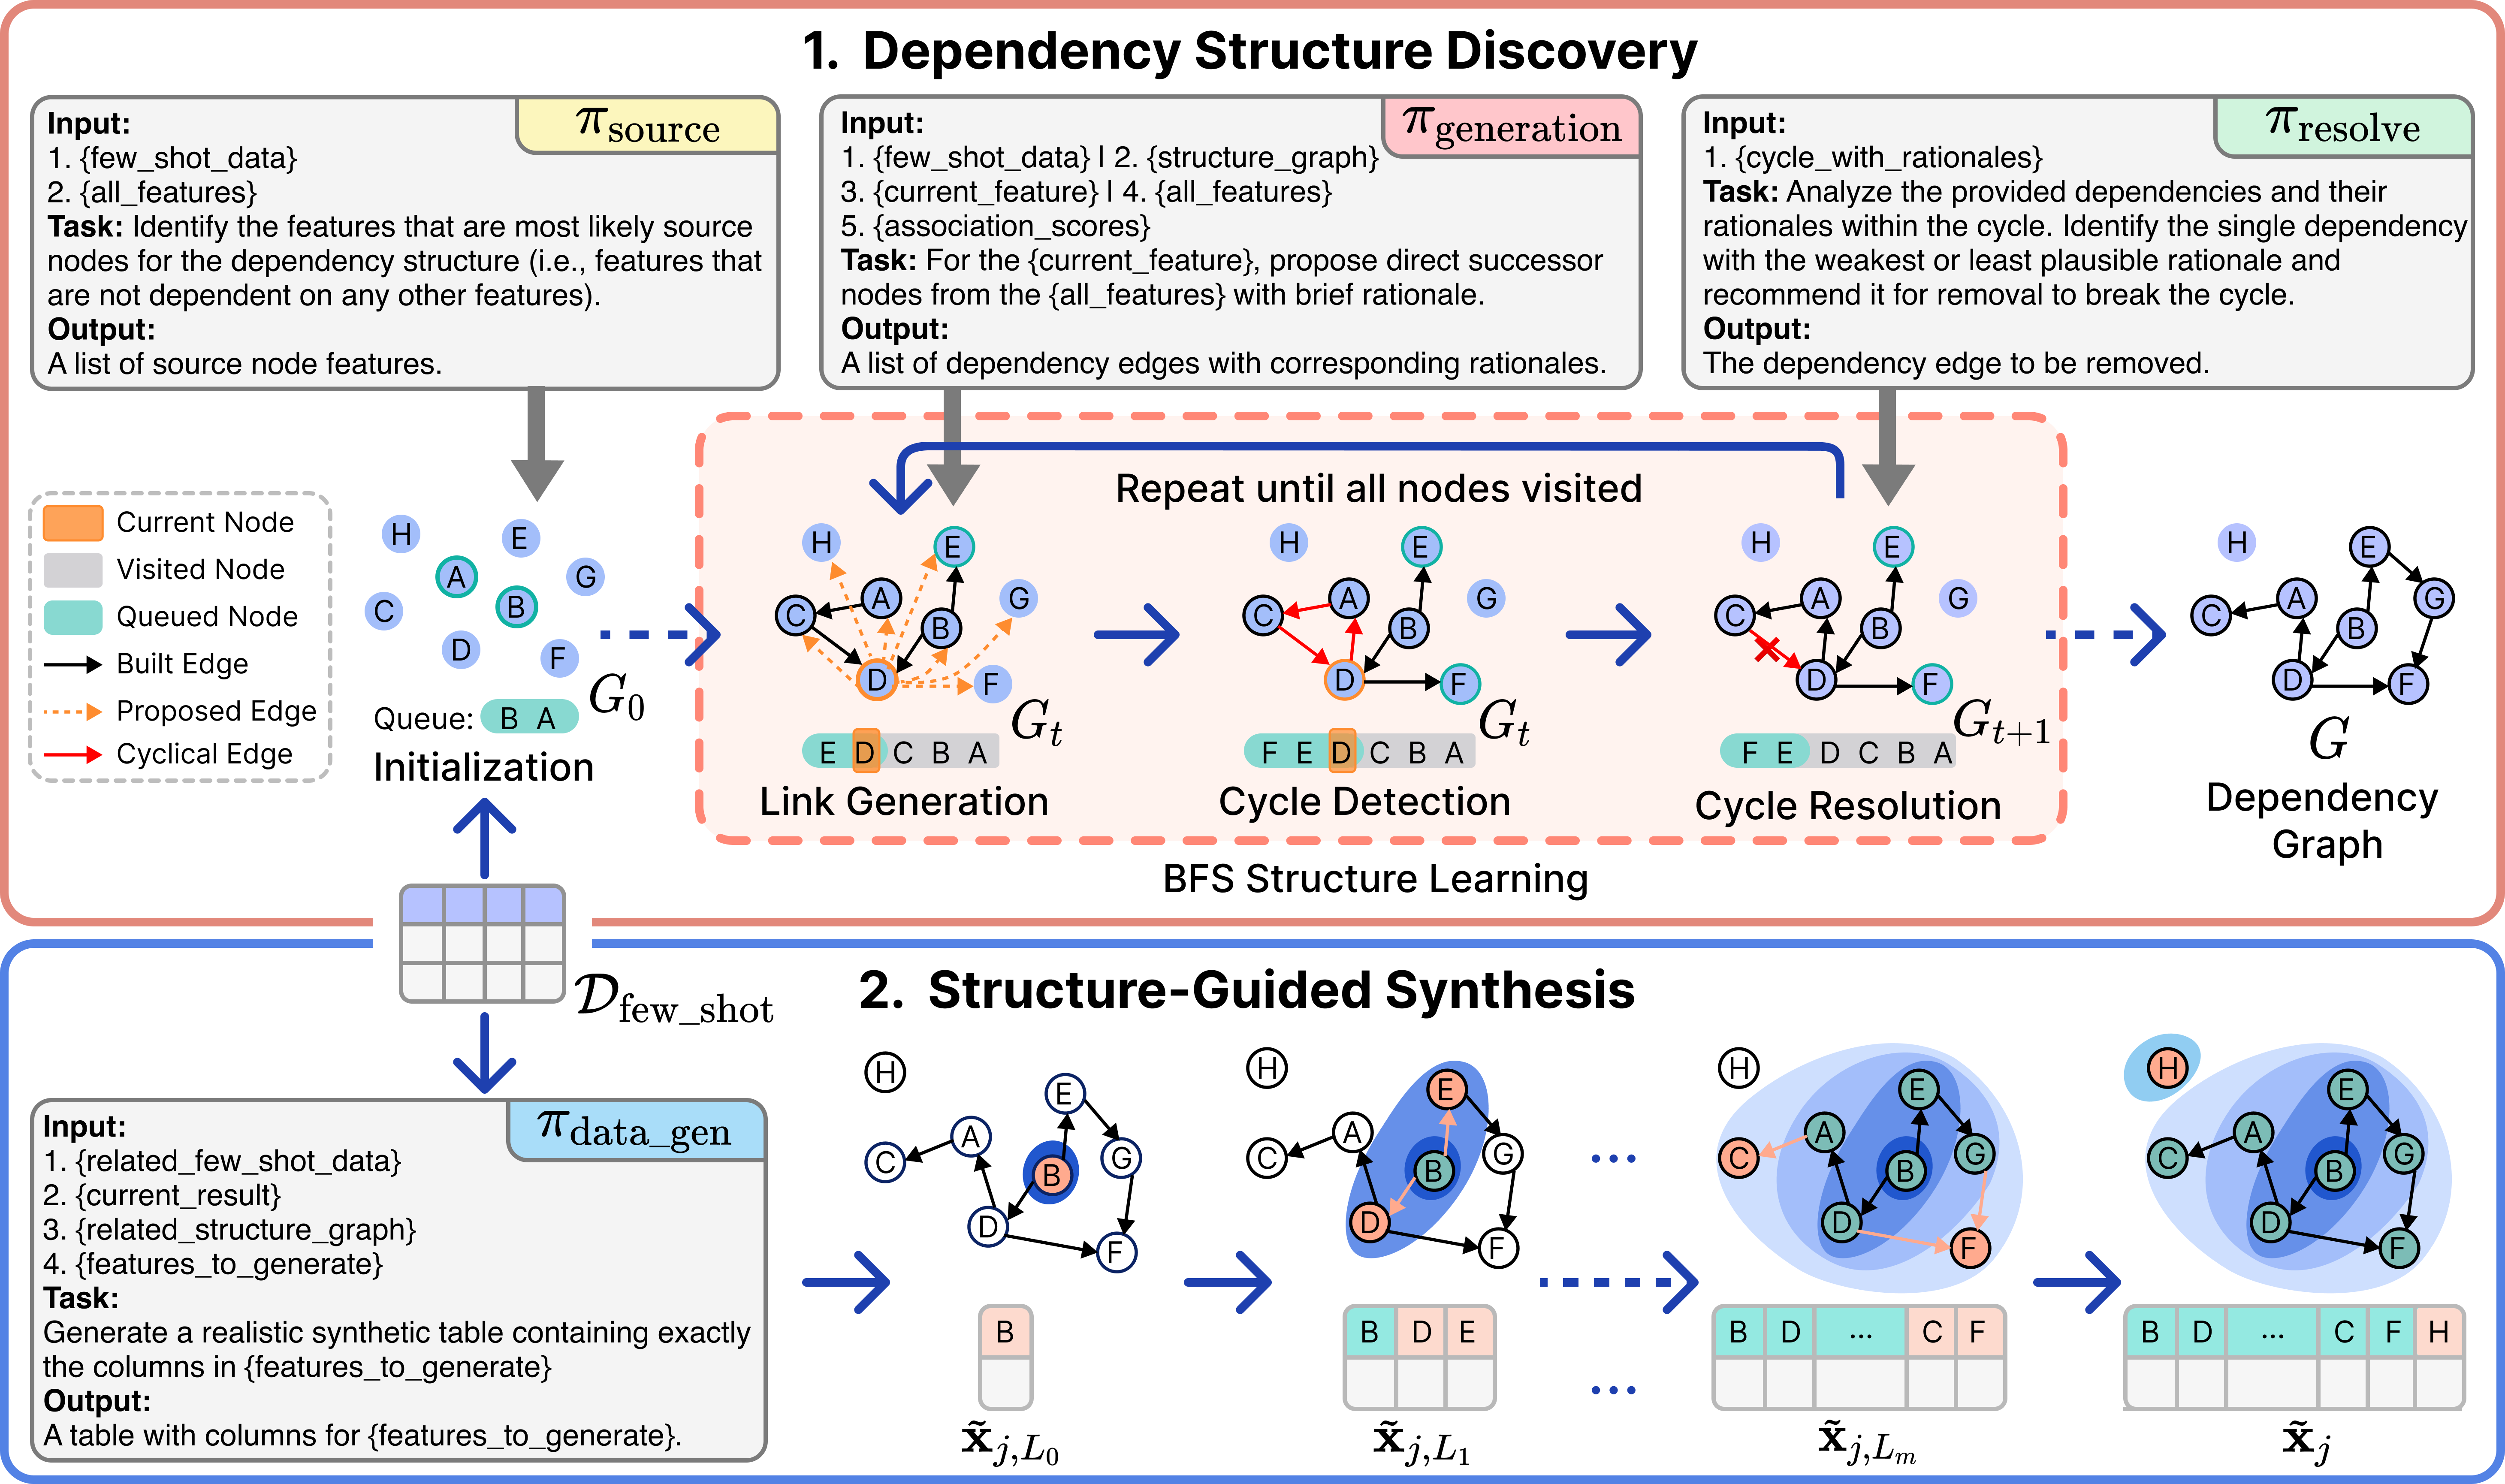
\includegraphics[width=\textwidth]{figures/pipeline.png}
\caption{Overview of the \textsf{StructSynth} framework. The method first performs \textbf{Dependency Structure Discovery} to infer a dependency graph from limited data via an LLM-guided search. Subsequently, \textbf{Structure-Guided Synthesis} leverages the learned graph as a blueprint to autoregressively guide the LLM in generating new tabular data.}
\label{fig:pipeline}
\end{figure*}

% \footnote{+yq+: shall we merge 2.1 and 2.2 and conventional methods?}

\subsection{Conventional Tabular Data Synthesis}
Tabular data synthesis addresses data scarcity and privacy concerns by learning generative models to sample realistic data. Early approaches, such as the SMOTE~\cite{chawla2002smote} and methods based on Copulas~\cite{xue2000multivariate}, were foundational but often struggled to capture complex, non-linear relationships.

\textbf{Deep Generative Models (DGMs).} This prompted a shift towards more expressive deep generative models (DGMs) that learn the data distribution implicitly. Advances in deep generative modeling, including Variational Autoencoders (VAEs) such as TVAE~\cite{patki2016synthetic}, Generative Adversarial Networks (GANs) exemplified by CTGAN~\cite{xu2019modeling}, and Normalizing Flow-based methods~\cite{papamakarios2021normalizing}, have significantly improved fidelity through implicit distribution learning. More recently, diffusion-based methods like TabDDPM~\cite{kotelnikov2023tabddpm} and TabSyn~\cite{tabsyn} achieved state-of-the-art performance. TabSyn, in particular, encodes mixed-type tabular data into a continuous latent space via VAE and applies score-based diffusion therein, explicitly improving inter-column relation fidelity while reducing inference steps. However, since these DGMs implicitly learn complex feature dependencies, they still offer limited interpretability and controllability over the generation process.

\textbf{Structure-Aware Methods.} To enhance generative fidelity and controllability, structure-aware methods explicitly incorporate feature dependency structures into data synthesis. Early methods based on Bayesian Networks~\cite{ankan2015pgmpy} and PrivBayes~\cite{zhang2017privbayes} generate samples guided by learned graphical structures, with PrivBayes introducing privacy-preserving mechanisms on top of the Bayesian framework. Recent deep-learning methods integrate structured inductive biases more effectively; DECAF~\cite{van2021decaf} leverages causal reasoning for fairness, while GOGGLE~\cite{liu2023goggle} employs a graph-based VAE. However, their effectiveness heavily depends on accurately learned graphs from data, posing challenges especially under limited data scenarios.


\subsection{LLM-Based Tabular Data Synthesis}
Large Language Models (LLMs), leveraging in-context learning and extensive prior knowledge, have recently advanced tabular data synthesis significantly. Fine-tuning approaches such as GReaT~\cite{borisov2023language}, TAPTAP~\cite{zhang2023generative}, and AIGT~\cite{zhang2025aigt} autoregressively generate data but incur high computational costs and deteriorate performance in low-data scenarios. Prompt-based methods, notably CuratedLLM (CLLM) \cite{cllm2024}, alleviate these drawbacks by using curated examples to guide data generation without updating model parameters. More recently, TabGen-ICL~\cite{fang-etal-2025-tabgen} further advances the prompting paradigm by iteratively selecting in-context examples that represent the residual between the real and currently generated distributions, achieving progressive distribution alignment without any model fine-tuning. Beyond prompting strategies, GraDe~\cite{zhang-etal-2025-features} addresses the structural mismatch between dense Transformer attention and sparse tabular dependencies by injecting a learned sparse dependency graph into the attention mechanism, guided by externally extracted functional dependencies; this graph-guided attention yields notable improvements on structurally complex datasets. Nevertheless, while these methods induce or integrate dependencies implicitly or locally, they do not yield an interpretable global dependency topology that can serve as an explicit, executable blueprint for structure-preserving generation~\cite{liu2024rethinking}.


\subsection{Structure Learning for Tabular Data}

\subsubsection{Conventional Structure Learning}
Conventional approaches to dependency structure discovery primarily fall into two categories: constraint-based and score-based methods. Constraint-based methods, such as the Peter--Clark (PC) algorithm~\cite{spirtes2000causation} and the Fast Causal Inference (FCI) algorithm~\cite{spirtes1995causal}, utilize conditional independence tests to iteratively prune edges from an initially fully connected graph. While PC assumes causal sufficiency (no hidden confounders), FCI is specifically designed to handle latent variables. In contrast, score-based methods optimize a global scoring criterion to identify the most suitable graph structure. A representative example is the Greedy Equivalence Search (GES)~\cite{chickering2002optimal}, which searches through equivalence classes to maximize a scoring function. However, both constraint-based and score-based approaches typically yield only Markov equivalence classes, thereby failing to distinguish between structurally distinct graphs that encode identical conditional independencies. To address this limitation, Functional Causal Models (FCMs) impose stronger assumptions regarding the data generation process. FCMs model effects explicitly as functions of direct causes combined with independent noise terms, enabling the identification of causal directions since independence between cause and noise typically breaks down when reversed~\cite{shimizu2006linear, hoyer2008nonlinear, zhang2009identifiability}. Recent advancements have generalized this approach, introducing conditions such as Generalized Independent Noise (GIN) to manage latent causal variables in linear, non-Gaussian settings~\cite{xie2020generalized}. However, the statistical power of these traditional algorithms heavily relies on a large number of samples, making them unreliable for structure discovery in the low-data regimes addressed by our work.

\subsubsection{LLM-based Structure Learning}
Leveraging Large Language Models (LLMs) for structure learning has recently emerged as a promising direction due to their inherent reasoning capabilities. Several paradigms have been proposed for integrating LLMs into structure discovery. Initially, methods focused on querying LLMs about pairwise causal relationships, showing strong accuracy in determining causal directions between variable pairs~\cite{kiciman2023causal}. To overcome the quadratic complexity inherent to pairwise approaches, more scalable methods employing breadth-first search (BFS) strategies have been introduced, reframing structure learning as a graph traversal task and significantly reducing the required number of queries to the LLM~\cite{jiralerspong2024efficient, zanna2025fairness}. A third paradigm enhances reliability by integrating an iterative supervision loop, in which traditional structure-learning algorithms propose initial graphs that are subsequently validated or corrected by LLMs. This method grounds LLM-generated structures in empirical evidence, thereby reducing hallucination risks~\cite{ban2023causal}. LLM-based structure discovery methods have demonstrated notable effectiveness across diverse domains, including medicine~\cite{naik2024applying, antonucci2023zero, arsenyan2024large}, economics~\cite{causal4financial}, and social sciences~\cite{manning2024automated}. Inspired by the success of LLMs in leveraging prior knowledge for domain-specific reasoning, our work integrates a scalable, LLM-driven paradigm for robust structure discovery.



